\chapter{Wykorzystane narzędzia i technologie}
\label{cha:wykorzystaneNarzedziaITechnologie}
W niniejszym rozdziale zostaną zawarte krótkie opisy narzędzi oraz technologii wykorzystanych w trakcie implementacji algorytmu będącego tematem owej pracy inżynierskiej. Zostanie również przedstawiony język programowania, w którym stworzono projekt, oraz jego zalety, które przeważyły o jego wyborze. 
\section{Python}
Język programowania Python \cite{PythonWiki} powstał we wczesnych latach dziewięćdziesiątych. Guido van Rossum jest uważany za głównego twórcę tego języka, jednak wkład w jego rozwój miały także inne osoby. 

Popularność narzędzia wzrosła diametralnie w momencie wydania wersji $2.0$ w roku 2000 i rośnie aż do teraz. Aktualnie znajduje się on w czołówce najczęściej wykorzystywanych języków. (Rys. \ref{fig:programmingLang}Jego interpretery dostępne są na wiele systemów operacyjnych, obsługuje większość używanych w dzisiejszych czasach platform, takich jak Windows, Linux, AIX, iOS i inne.

\begin{figure}[h]
	\centering
	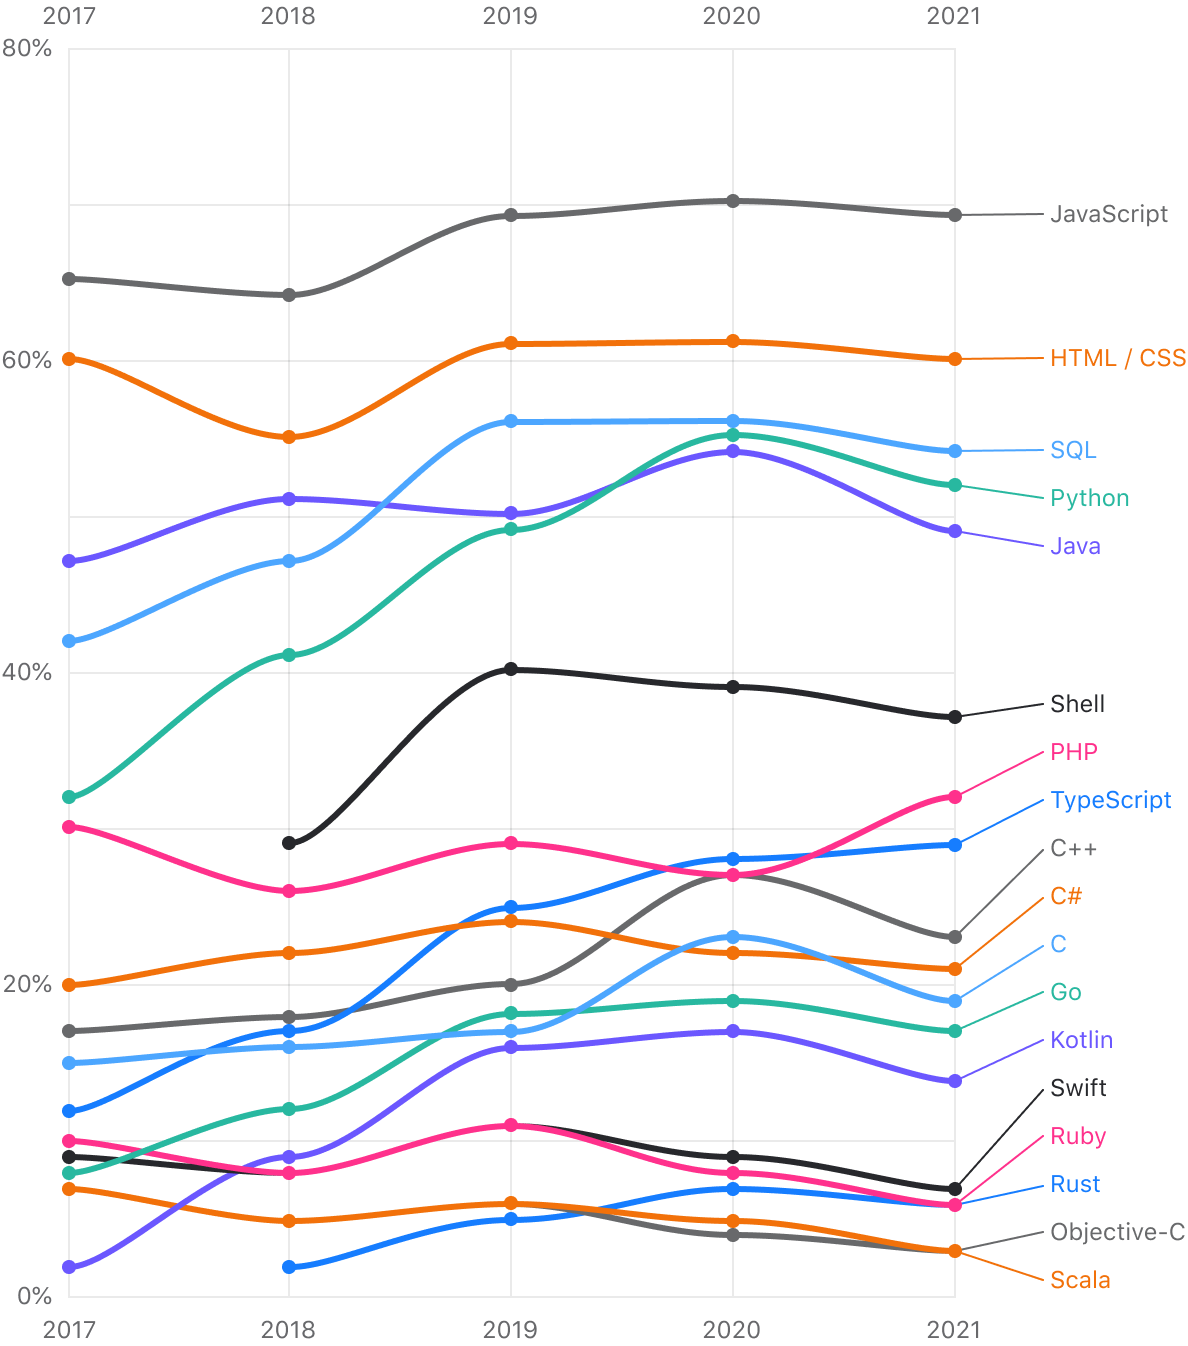
\includegraphics[width=7cm]{python.png}
	\caption{Popularność wybranych języków programowania na przestrzeni lat.} 
	\label{fig:programmingLang}
\end{figure}

Projekt w ramach którego rozwijany jest owy język zarządzany jest przez organizację Python Software Foundation. Narzędzie uznawane jest jako Open Source, toteż celem organizacji nie jest przyniesienie zysków osobom zarządzającym. 

Python jest językiem wielopoziomowym, którego przeznaczenie nie jest ściśle określone. Jego możliwości są niezwykle rozległe i uzależnione od stosowanych bibliotek, platform oraz gotowych skryptów, których wybór jest wyjątkowo obszerny. 

Język nie wymusza od użytkownika jednego stylu, w którym tworzone są programy. Istnieje możliwość zastosowania różnych paradygmatów programowania (obiektowe, strukturalne oraz funkcyjne), co zdecydowanie wpływa na rozległość jego zastosowań. Ważną kwestią jest także jego dynamiczność, podczas tworzenia zmiennych nie wymaga się definiowania ich typu. Co więcej Python posiada automatyczne zarządzanie pamięcią, które zwalnia programistę z tego obowiązku. 

Główna idea towarzysząca twórcy podczas opracowywania jego składni była wysoka czytelność kodu źródłowego, jego przejrzystość i zwięzłość. Okazało się to jednym z głównych czynników, które spowodowały, że stał się tak powszechnie stosowany.

Dzięki swojej uniwersalności i wygodnym zastosowaniom Python zostaje używany w wielu różnych dziedzinach (Rys. \ref{fig:pythonUsage}). Popularność w środowisku matematycznym zawdzięcza środowisku SciPy stanowiącą darmową alternatywę do języka Matlab. 

\begin{figure}[h]
	\centering
	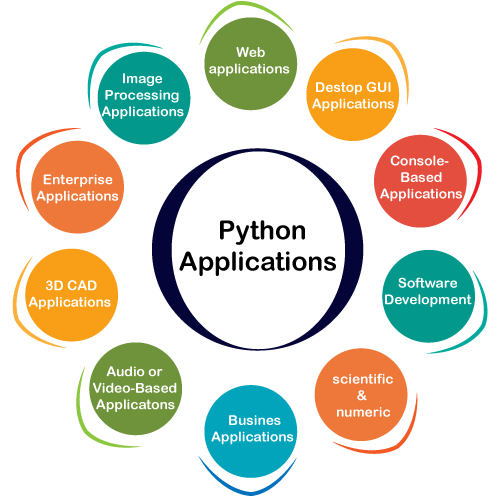
\includegraphics[width=7cm]{python_usage.png}
	\caption{Dziedziny, w których najczęściej wykorzystuje się język programowania Python.} 
	\label{fig:pythonUsage}
\end{figure}

Biblioteka Tensor Flow wspiera tworzenie sieci neuronowych, co znajduje zastosowanie w tworzeniu algorytmów wykorzystywanych w popularnych aplikacjach. \cite{PythonApps} W przypadku dziedzin operujących na przetwarzaniu obrazów czy też analizowaniu danych Python dostarcza kilka bibliotek ułatwiających te operacje. W następnym podrozdziale zostaną przedstawione biblioteki użyte w implementacji animacji awatara.

\section{Biblioteki}
Biblioteki programistyczne dostarczają podprogramy, które użytkownik może wykorzystać w swoim kodzie źródłowym bez konieczności implementowania ich od podstaw. Jest to metoda na wielokrotne używanie identycznego kodu.

\subsection{OpenCV}
Biblioteka OpenCV \cite{opencv} jest narzędziem wydanym jako otwarte oprogramowanie, wspomagające przetwarzanie obrazów oraz uczenie maszynowe. Została napisana w języku C, natomiasto posiada interfejsy dla innych języków, takich jak Java, Python bądź Matlab.

Zawiera około 2500 zoptymalizowanych algorytmów implementujących między innymi wykrywanie i rozpoznawanie twarzy, identyfikację i śledzenie ruchu obiektów. Znajdują się w niej także moduły dotyczące modeli 3D, ich tworzenia i przetwarzania.

Poza skomplikowanymi algorytmami OpenCV dostarcza wiele podstawowych operacji, które wykorzystuje się przy modyfikacji obrazów. Zaimplementowane funkcje zdają się wyróżniać wydajnością, co jest bardzo istotne w przypadku działania na dużych zbiorach danych.

\subsection{imutils}
Pakiet imutils \cite{imutils} to kolejne przydatne narzędzie w trakcie modyfikacji obrazów. Zawiera szereg funkcji ułatwiających ich przetwarzanie, takich jak obracanie, zmiana rozmiaru, przesunięcie, zastosowanie szkieletyzacji. Zaimplementowano także moduły ułatwiające poprawną prezentację zdjeć podczas ich wyświetlania.

Funkcje zawarte w owym pakiecie pochodzą z biblioteki OpenCV, zostały one odpowiednio połączone i zmodyfikowane, aby można było w prostszy sposób dokonywać podstawowych operacji na zdjęciach. Biblioteka OpenCV zawiera ogromną ilość komponentów, co może być przytłaczające dla osoby rozpoczynającej swoją przygodę z przetwarzaniem obrazów.

Ideą, dla której powstał tenże pakiet była chęć zebrania podstawowych modułów i odpowiednie ich dostosowanie w celu ograniczenia zbędnych operacji, które należy zastosować korzystając z biblioteki OpenCV.

\subsection{dlib}
Dlib to biblioteka udostępniona na zasadach otwartej licencji, napisana w języku C++. Dostarczająca algorytmy oparte o uczenie maszynowe oraz narzędzia do tworzenia oprogramowania we wspomnianym wyżej języku. 

Funkcje, z których można korzystać implementują algorytmy trenujące takie klasyfikatory jak SVM, SVR czy też klasyfikację bez nadzoru. Dodatkowo istnieje możliwość wytrenowania własnego modelu wykrywającego twarz lub jej punkty charakterystyczne.

Zastosowania tej biblioteki obejmują takie dziedziny jak przemysł, robotyka oraz wszelkie obszary wymagające skorzystania z programów o dobrej wydajności obliczeniowej.

\subsection{skimage}
Biblioteka scikit-image \cite{skimage}, podobnie jak opisane powyżej pakiety, zawiera szereg implementacji algorytmów powiązanych z przetwarzaniem obrazów. Została udostępniona jako otwarte oprogramowanie tworzone przez kilkadziesiąt osób. 

Obejmuje ona takie algorytmy jak transformacje, segmentację obrazów, ich morfologię oraz manipulację przestrzenią kolorów. Pakiet korzysta z tablic biblioteki NumPy, wykorzystanych do przechowywania obrazów.


\section{Flask}
\section{Pycharm}